
\section{Wednesday}\index{Wednesday_lecture}
\subsection{Application}
\paragraph{Mixture problem}There are two things that you need to bear in mind: \\\textcolor{red}{$\frac{\diff y}{\diff t}=$ input rate - output rate}, carry the units.

\begin{example}
A 120-gal tank initially contain 90kg salt dissoved in 90-gal of water. Brine containing 2kg/gal of salt flows into the tank at the water. Brine containing 2kg/gal of salt flows into the tank at the rate of 4gal/min, \& the well-stirned mixture flows out at the rate of 3 gal/min. How much salt does the tank contain when it is full?
\begin{figure}[H]
\centering
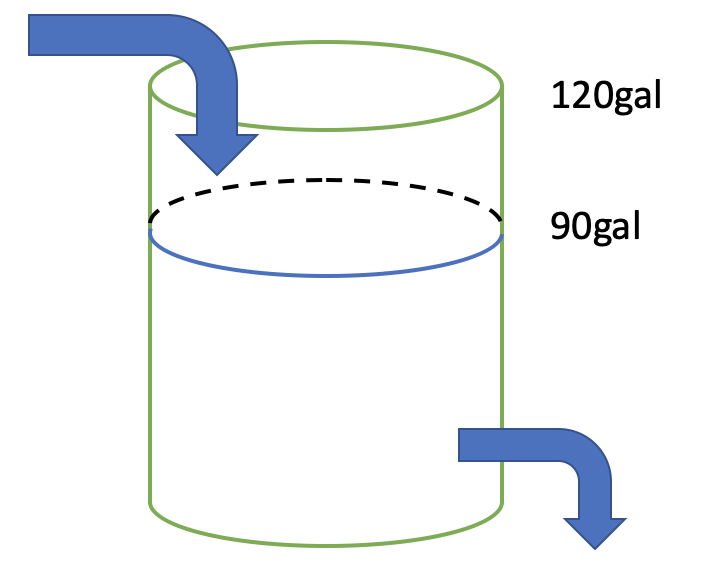
\includegraphics[width=5cm]{week2_wed_first}
\caption{First}
\end{figure}
Set $y(t)=$ the amount of salt at time $t$,\\ $V(t)=$the amount of brine at time $t$= 90 +$t$(gal)(t:minute)\\
\[\begin{aligned}y^\prime(t)&=2\text{kg/gal}\cdotp4\text{gal/min}-\frac{y(t)}{V(t)}\text{kg/gal}\cdotp3\text{gal/min}\\
&=8\text{kg/min}-3\frac{y(t)}{V(t)}\text{kg/min}
\end{aligned}
\]
\[y^\prime=8-3\frac{y}{90+t}
\]
\[y^\prime+\frac{3}{90+t}y=8
\]
By intergrating factor,
\[(e^{\int\frac{3}{90+t}\diff t}\cdotp y)^\prime=8e^{\int\frac{3}{90+t}\diff t}
\]
Try to simplify $e^{\int\frac{3}{90+t}\diff t}$;
\[\begin{aligned}\int\frac{3}{90+t}\diff t&=3ln|90+t|+\tilde{c}\\&=3ln(90+t)+\tilde{c}\end{aligned}
\]
Then,
\[e^{\int\frac{3}{90+t}\diff t}=(90+t)^3\cdotp c
\]
Integrate both sides,
\[(90+t)^3\cdotp c\cdotp y=8\int(90+t)^3\cdotp c\diff t
\]
\[(90+t)^3y=2\cdotp(90+t)^4+C
\]
\[y=2(90+t)+\frac{c}{(90+t)^3}
\]
\[y(0)=90=180+\frac{c}{90^3}\quad\Rightarrow\quad c=-90^4
\]
\[y=2(90+t)-\frac{90^4}{(90+t)^3}
\]
At $t=30$ the tank is full \& $y(30)=240-\frac{90^3}{120^3}\cdotp90$
\end{example}

\begin{example}[Persuit problem]
In a naval excercise, a distroyler $D$ is hunting a submarine $S$. Suppose $D$ at $(9,0)$ detects $S$ at $(0,0)$ \& at the same time $S$ detects $D$. Assuming that $S$ will dive immediately \& depart at full speed, $15$mile/hr in a straight course of unknown direction. What path should the destroyer $D$ follows to be certain of passing directly over the submarine $S$. If the speed of $D$ is $30$mile/hr at all time of the pursuit?
\begin{figure}[H]
\centering
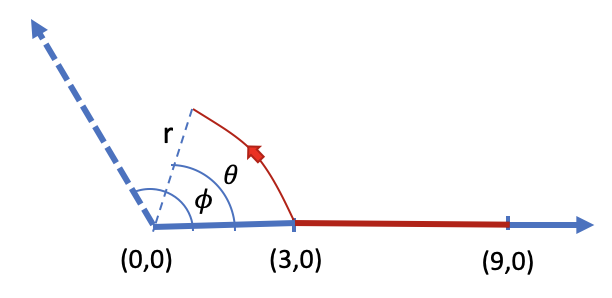
\includegraphics[width=8cm]{week2_wed_sec}
\caption{The path of destroyler in red.}
\end{figure}
Distance $D$ has travelled=$6+\int_0^\phi\sqrt{(r(\theta))^2+(r^\prime(\theta))^2}\diff\theta$.\\
Distance $S$ has travelled=$r(\phi)$.\\
For the speed of $D$ is twice than that of $S$, with the same period of time:
\[6+\int_0^\phi\sqrt{(r(\theta))^2+(r^\prime(\theta))^2}\diff\theta=2r(\phi)
\]
This isn't a form that can be dealt with. Differentiate both side,
\[\sqrt{(r(\phi))^2+(r^\prime(\phi))^2}=2r^\prime(\phi)
\]
\[(r(\phi))^2+(r^\prime(\phi))^2=4(r^\prime(\phi))^2
\]
\[r^\prime(\phi)=\pm\frac{1}{\sqrt{3}}r(\phi)
\]
W.L.O.G pick plus sign $\frac{r^\prime}{r}=\frac{1}{\sqrt{3}}$
\[lnr=\frac{1}{\sqrt{3}}\phi+\tilde{c}
\]
\[r=e^{\frac{\phi}{\sqrt{3}}}\cdotp c
\]
\[r(0)=3=c
\]
\[r(\phi)=3e^{\frac{\phi}{\sqrt{3}}}
\]
Given the direction $S$ take $\phi$, if $D$ want to be above it, they would reach each other at $(\phi,3e^{\frac{\phi}{\sqrt{3}}})$. This implies that if $D$ follows the path of 
$r(\theta)=3e^{\frac{\theta}{\sqrt{3}}}$, $D$ can catch $S$ whichever direction $S$ take.
\end{example}
\begin{remark}
There is a link about basic idea of how to compute the length of a curve:
\href{http://tutorial.math.lamar.edu/Classes/CalcII/ArcLength.aspx}{http://tutorial.math.lamar.edu/Classes/CalcII/ArcLength.aspx}. Check it if you are interested.
\end{remark}
\paragraph{Orthoganal trajectories} Given a family of curve $f(x,y,c)=0$. To find its orthoganal trajectories, the slope of the graph is needed. Differentiate $F$ by $x$;
\[F_x+F_yy_x=0
\]
Slope is $y_x=-\frac{F_x}{F_y}$. Then the slope of the graph that is orthoganal to the original one is \[y_x=\frac{F_y}{F_x}=\frac{\frac{\partial F}{\partial y}(x,y,c)}{\frac{\partial F}{\partial x}(x,y,c)}\]
\begin{example}
$y=cx^2$ $c$:parameter. To find another family of curves which is orthoganal to $y=cx^2$ whenever they intersect with each other.\\
$y=cx^2$, $\frac{\diff f}{\diff x}=2cx$ O.T. $\rightarrow \frac{\diff f}{\diff x}=\frac{-1}{2cx}=\frac{-1}{2\frac{y}{x^2}x}=-\frac{x}{2y}$ ( A separable equation)\\
$2y\diff y+x\diff x=0\quad\rightarrow\quad y^2+\frac{1}{2}x^2=c$
\end{example}


